\section*{Annexes}
\addcontentsline{toc}{section}{Annexes}

\label{resultCanny}
\begin{figure}[H]
  \center
 \begin{tabular}{|c|c|}
  \hline
  image originale & image après filtre de Canny\\
  \hline
  
\includegraphics{image/original.png} & 
\includegraphics{image/canny_final.png}\\
  \hline
  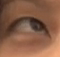
\includegraphics{image/original_asiatique.png} & 
\includegraphics{image/cannyAsiatique.png}\\
  \hline
  
\includegraphics{image/original_black.png} & 
\includegraphics{image/cannyBlack.png}\\
  \hline
 \end{tabular}
  \caption{Résultats du filtre de Canny sur des personnes de couleur de peau différentes}
\end{figure}



\newpage